This section gives you a very basic idea of how to get started with
simple tasks.  To run the following examples, you will first need to:
\begin{itemize} 
\item Install the LSST software stack on your machine.
Appendix~\ref{appendix-stackinstall} describes how to do this.
\item Make sure that you have defined the LSST\_HOME environment
variable.
\item Source \$LSST\_HOME/loadLSST.csh or \$LSST\_HOME/loadLSST.sh
from your shell
\item At your shell prompt, type \texttt{setup
afw}. Appendix~\ref{appendix-stackinstall} explains more about the
purpose of the \texttt{setup} command.
\item Optionally, configure Python to remember
your command history and provide word completion; see
Appendix \ref{appendix-interactivePython}.
\item Type \texttt{python} to start the python interpreter, and copy/paste the examples in.
\item If you are unfamiliar with object-oriented programming lingo,
read or consult Appendix~\ref{appendix-lingo} as necessary.  
\end{itemize} 

\section{Reading and displaying a FITS image}

The main package we'll be using is the \texttt{afw} (applications
framework) package, so we start by importing some afw subpackages.
%Remember to \texttt{setup afw} at your Unix prompt after sourcing
%loadLSST.csh but before starting Python (see the end of
%Appendix~\ref{appendix-stackinstall} if you're not sure why).

\begin{verbatim}
import lsst.afw.display.ds9 as ds9
import lsst.afw.image as afwImg

im1 = afwImg.ImageF(`image1.fits')
ds9.mtv(im1, frame=0)
\end{verbatim}

Use the name of any handy FITS image in place of image1.fits.
\texttt{ImageF} creates an image of floats, \texttt{ImageD} creates an
image of doubles.  If you do not already have ds9 running, Python will
start it for you at this point.

\section{Image arithmetic}

To save memory and time, images are operated on in-place.  That is,
you can subtract images of identical size like this:

\begin{verbatim}
import lsst.afw.display.ds9 as ds9
import lsst.afw.image as afwImg

im1 = afwImg.ImageF(`image1.fits')
im2 = afwImg.ImageF('image2.fits')

im1 -= im2
\end{verbatim}

Be careful: this modifies im1!  If you were looking to do something
like \texttt{im3=im1-im2}, where im3 is a new image, you must
explicitly force the creation of the new image and {\it then} do the
in-place arithmetic:

\begin{verbatim}
import lsst.afw.display.ds9 as ds9
import lsst.afw.image as afwImg

im1 = afwImg.ImageF(`image1.fits')
im2 = afwImg.ImageF('image2.fits')

im3 = afwImg.ImageF(im1,True) # create deep copy
im3 =- im2
\end{verbatim}

Again, this is because when working with large amounts of data we want
to minimize the amount of pixel copying.  The system is designed to
avoid new copies unless explicitly asked.  The penultimate line
creates a new copy of im1, called im3.  Setting the second argument
to \texttt{True} is necessary to make a {\it deep copy}, meaning that
the resulting image is a completely new image, independent of the
parent image and occupying its own area of memory.  If the second
argument is \texttt{False} or is omitted, a shallow copy is generated,
meaning that the copy {\it still refers to the pixel values stored in
the parent image}.  Thus, if the pixels of a shallow copy are
modified, the corresponding pixels in the parent image will be
modified as well.  {\it Astronomers who are new to the concept of deep
and shallow copies will want to pay particular attention to this
point.}  Shallow copies save memory and time (for example, making
postage stamps from a large image can be very fast and efficient) but
you must handle them properly (don't modify the postage stamps if you
will need to refer to the original pixel values).

%\item If you are not familiar with object-oriented programming, you
%  may be surprised to see that the ``function'' \texttt{ImageF}, which
%  was previously called with a string (the filename) as its first and
%  only argument, is now being called with {\it two} arguments, the
%  first of which is not even a string.  This is a powerful
%  feature. Conceptually, we know that an image can be constructed in
%  many different ways.  However, many programming languages in the
%  past forced us to declare different names for procedures which
%  operate on different data types or take different numbers of
%  arguments, even if they are conceptually similar.  With C++ and
%  Python, conceptually similar operations can have the {\it same
%    name}.  \texttt{ImageF} is not really a function; in
%  object-oriented lingo it is a called a {\it method}.  Because it
%  makes a new object, it is more specifically called a {\it
%    constructor}.  We will soon see how to browse the C++
%  documentation for all the different ways to construct an image.
%\end{itemize}

Similar operators \texttt{+=}, \texttt{*=}, and \texttt{/=} are
defined, which do the obvious things.  The object on the right-hand
side can also be a scalar rather than an image.

\section{Cutting, copying, pasting, and writing images}

To cut out a sub-image, we must first create a \texttt{BBox} or
bounding box object, which itself must be defined by two
\texttt{PointI}\footnote{\texttt{PointI} defines a point where the
 coordinates are integers, hence the ``I''.}  objects which specify
the corners.  We then call \texttt{ImageF} in a new way:

\begin{verbatim}
import lsst.afw.image as afwImg

im1 = afwImg.ImageF(`image1.fits')

llc = afwImg.PointI(290,250)
urc = afwImg.PointI(300,260)
bbox = afwImg.BBox(llc,urc)
im4 = afwImg.ImageF(im1,bbox,False)
\end{verbatim}

\texttt{llc} and \texttt{urc} define the lower left and upper right
corners of the bounding box, respectively.  This form of the
\texttt{ImageF} constructor takes an image as its first argument, a
bounding box as its second argument, and thirdly the boolean
indicating the type of copy (\texttt{False} indicating that a deep
copy should not be made).  Shallow copies are excellent for
efficiently extracting postage stamps, as long as you remember the
implications of modifying their pixel values.

You can set pixel values using the \texttt{<<=} operator.  For
example, if you wanted to set all the pixels inside the bounding box to a
scalar value, say 99:

\begin{verbatim}
im4 <<= 99
\end{verbatim}

This also works if the right-hand side is an image of the correct size.

You can also easily mosaic images together.  The following example
makes a new mosaic image in memory and displays it.  This would be
useful for making a picture gallery of interesting galaxies, for
example.

\begin{verbatim}
import lsst.afw.image as afwImg
import lsst.afw.display.utils as utils

im1 = afwImg.ImageF(`image1.fits')
im2 = afwImg.ImageF(`image2.fits')
im3 = afwImg.ImageF(`image3.fits')
im4 = afwImg.ImageF(`image4.fits')

images = [im1, im2, im3, im4]
labels = [`Label 1', `Label 2', `Label 3', `Label 4']

m = utils.Mosaic()
m.setMode(`square')
m.setGutter(0)

mosaic = m.makeMosaic(images)
ds9.mtv(mosaic, frame=0)
m.drawLabels(labels, frame=0)
\end{verbatim}

In the \texttt{setMode} command, the default is ``square'' which will
make the mosaic image as square as possible.  Other allowed values are
``y'' and ``x'' which make the mosaic one image wide and one image
high, respectively.  The \texttt{setGutter} command sets the number of
pixels between each image in the mosaic.

To save your mosaic image as a new FITS file:

\begin{verbatim}
afwImg.ImageF.writeFits(mosaic,'filename.fits')
\end{verbatim}


\section{Image statistics}

\texttt{math.makeStatistics} computes image statistics and returns an
object which you can then query for the statistics you want.  To save
computation time, you specify beforehand which statistics to compute,
as follows:

\begin{verbatim}
import lsst.afw.image as afwImg
import lsst.afw.math as math

im1 = afwImg.ImageF(`image1.fits')

flags = math.MEAN | math.STDEV | math.ERRORS 
stats = math.makeStatistics(im1,flags)

print stats.getResult(math.STDEV) # prints stdev AND its uncertainty
print stats.getResult(math.MEAN) # ditto for mean

\end{verbatim}

Possible statistics to calculate:
\begin{itemize}
\item ERRORS     include errors of requested quantities.
\item NPOINT     number of sample points
\item MEAN     estimate sample mean
\item STDEV     estimate sample standard deviation
\item VARIANCE     estimate sample variance
\item MEDIAN     estimate sample median
\item IQRANGE     estimate sample inter-quartile range
\item MEANCLIP     estimate sample N-sigma clipped mean
\item STDEVCLIP     estimate sample N-sigma clipped stdev
\item VARIANCECLIP     estimate sample N-sigma clipped variance
\item MIN     estimate sample minimum
\item MAX     estimate sample maximum
\item SUM     find sum of pixels in the image
\item MEANSQUARE     find mean value of square of pixel values
\item NOTHING     We don't want anything.
\end{itemize}

This list is provided here to give you an idea of the capabilities in
the system, but capabilities change over time.  It's a good idea to
check the C++ documentation (as described below) for the most
up-to-date list.  
% Introduce this idea in the next section
%The main selling point is not that you can compute
%statistics---many software packages can do that---but that if you use
%\texttt{maskedImage}s, the masks are {\it automatically applied} when
%computing the statistics.

If you want detailed control over how the statistics are computed, for
example changing the clipping from the default 3$\sigma$ and 3
iterations, you must create a StatisticsControl object with five
arguments: the number of sigma to clip at, the number of iterations
for clipping, a specification of which bitplanes of the mask to use (0
means use all of them; mask bitplanes will be explained in the next
section, and in this case we have no mask yet anyway), a boolean
indicating whether to avoid using pixels which have NaN (not-a-number)
values, and a boolean indicating whether to weight pixels by their
inverse variance.  In the example below, we use all the default values
except to ask for 5$\sigma$ rather than 3$\sigma$ clipping.

\begin{verbatim}
import lsst.afw.image as afwImg
import lsst.afw.math as math

im1 = afwImg.ImageF(`image1.fits')

flags = math.MEAN | math.STDEV | math.ERRORS 
stats = math.makeStatistics(im1,flags)

ctrl = math.StatisticsControl(5.0,3,0,True,False)
stats = math.makeStatistics(im1,flags,ctrl)
print stats.getResult(math.STDEV) 
\end{verbatim}

In this case, we get a larger STDEV because we clipped less harshly
than the default.


\section{Masked images}

So far this may seem rather mundane, but the framework has some
features that will make it much more powerful with almost no extra
work on your part.  For example, we often want to propagate
uncertainties through these arithmetic operations, and apply masks
which ensure that the operations are not done on bad areas of the
image.  The applications framework defines a \texttt{maskedImage}
which contains an image, a variance image, and a mask image.
Once you have constructed \texttt{maskedImage}s, masking and
uncertainty propagation is done {\it automatically} when you invoke
these arithmetic operations.

Before the examples, a few remarks about masks are in order:
\begin{itemize}
\item The mask part of MaskedImage has pixels of type unsigned, so is
  created with the lsst.afw.image.MaskU constructor.  However, you may
  not need to specifically create the mask, because there are other
  constructors, such as lsst.afw.image.MaskedImageF, which will create
  both the data image (float in this case) and the mask in one call.
\item The mask is quite flexible, far more than just a binary one or
  zero indicating a good or bad pixel.  It has 16 bitplanes, and you
  can assign any meaning you want (eg, saturated, bad pixel, etc) to
  any of the planes.  In this manual, we will stick to the default set
  of planes:
\begin{verbatim}
Plane 0 -> BAD
Plane 1 -> SAT
Plane 2 -> INTRP
Plane 3 -> CR
Plane 4 -> EDGE
Plane 5 -> DETECTED
Plane 6 -> DETECTED_NEGATIVE
\end{verbatim}
% LIST HERE??  
In fact, we do not have to worry about which plane is
  assigned which meaning because we can always use getters and setters
  to manipulate data by meaning rather than by plane number.
\end{itemize}

% I'm not sure this example is instructive:
%To create a masked image from nothing, use the following example, substituting your own dimensions for the ones included here.
%
%\begin{verbatim}
%import lsst.afw.image as afwImg
%
%a = afwImg.ImageF(10,10) # image
%v = afwImg.ImageF(a.getDimensions()) # variance image
%m = afwImg.MaskU(a.getDimensions()) # mask
%mi = afwImg.MaskedImageF(a,m,v) # put it all together into one maskedImage
%\end{verbatim}

%That last line is a bit of a bore as you have to remember the \verb|F|;  fortun%ately you can get the computer to do the work by saying
%\begin{verbatim}
%mi2 = afwImg.makeMaskedImage(a, m, v)
%\end{verbatim}

Let's create an artificial masked image and then show how it works.
First, we'll demonstrate that variances automatically propagate
correctly when we do math operations on a MaskedImage (remember,
having a mask is not the only key feature of a MaskedImage; the
variance image is also useful and powerful).

\begin{verbatim}
import lsst.afw.image as afwImg

im1 = afwImg.MaskedImageF(100,100) # new 100x100 masked image
                                   # with zero pixel vals in data,
                                   # variance, and mask images

# set the variance to something nonzero
vari = im1.getVariance()
vari.set(1.0)  # this sets ALL pixels of the variance image

# the variance should increase by 4 if we multiply
# the data by 2
im1 *= 2
vari.get(0,0) # we just look at the 0,0 pixel because they're
              # all the same at this point
\end{verbatim}

The result is a variance of 4, as it should be. Let's try operations
involving two images:
\begin{verbatim}
import lsst.afw.image as afwImg

im1 = afwImg.MaskedImageF(100,100) 
im2 = afwImg.MaskedImageF(100,100) 

# set the variances to something nonzero
var1 = im1.getVariance()
var1.set(1.0)
var2 = im2.getVariance()
var2.set(2.0)

# the variances should add when we add or multiply the images
im1 += im2
var1.get(0,0) 
\end{verbatim}

The variance is now 3; the variances automatically added when I added
two images.  Note that {\it multiplying} these images would result in
zero variance because propagation of errors through multiplication
involves multiplying by the pixel values themselves, which are zero
here.  To convince yourself that variances are propagated through
multiplication correctly, you might want to set the pixels to nonzero
values.

Now let's simulate a saturated pixel and show how the mask
autmatically excludes it from the statistics:

\begin{verbatim}
import lsst.afw.image as afwImg
import lsst.afw.math as math

# set up our usual image with zero pixvals and unit variance
im1 = afwImg.MaskedImageF(100,100) 
var1 = im1.getVariance()
var1.set(1.0)

# set one saturated pixel
img = im1.getImage()
img.set(0,0,65000.0) # this sets just the 0,0 pixel

# get statistics BEFORE masking
stats = math.makeStatistics(im1,math.MEAN|math.NPOINT|math.STDEV)
stats.getResult(math.MEAN)
stats.getResult(math.STDEV)
stats.getResult(math.NPOINT)

# over 10000 pixels, the mean is 6.5 and the stdev is 650,
# because of the one saturated pixel (the rest are zero)

# if you want to visualize the image we created
import lsst.afw.display.ds9 as ds9
ds9.mtv(im1)

# now mask the saturated pixel
mask = im1.getMask()
satbit = mask.getPlaneBitMask('SAT')
mask.set(0,0,satbit) # again, setting just the 0,0 pixel

# and try the statistics again
stats = math.makeStatistics(im1,math.MEAN|math.NPOINT|math.STDEV)
stats.getResult(math.MEAN)
stats.getResult(math.STDEV)
stats.getResult(math.NPOINT)

# now, over 9999 pixels, the mean and variance are zero
\end{verbatim}

So once you have masked your pixels and defined your variances, the
framework makes math operations on images extremely useful because
the masking and variance propagation happen automatically.  In real
life, you will not be manually setting mask bits and variances.  We
will cover more realistic examples in later chapters, but this should
be enough to demonstrate the usefulness of the framework.

Note: because you are running interactively,
stats.getResult(math.WHATEVER) prints the result.  In a real script,
you would store the result for later use with something like
\texttt{mean = stats.getResult(math.MEAN)}.


\section{Exposures}

As you have probably already noticed, calling an object an ``image''
in the LSST environment is not as simple as it sounds - there are
several classes which in everyday English could all be called images,
but which behave differently in the LSST software.  The image on the
following page charts their relationships.

To begin, an ``image'' is simply a 2D array of pixels. A MaskedImage
includes an image, a variance image, and a mask, as already explained.
An Exposure is what you will most likely actually be working with.  It
aggregates a MaskedImage and a few other useful things: 
\begin{itemize}
\item Metadata, or information about the data.  You can think of this
  as a sort of ``FITS header'', but it is far more flexible because it
  is really a Python dictionary.
\item An optional point-spread function (PSF).  We'll see later how to
  generate and use this.
\item An optional World Coordinate System (WCS) which maps pixel
  locations to (usually) RA and DEC. We'll see later how to generate
  and use this.
\end{itemize}

You can construct an Exposure from a FITS file with\footnote{Note the
  templating: it is ExposureF in Python even though in C++ Exposure is
  templated over the types of image, mask, {\it and} variance:
  \texttt{Exposure< ImageT, MaskT, VarianceT >}.  In other words, if
  you read the C++ documentation you might have expected to use
  ExposureFUF.  To simplify life in Python, only ExposureF and
  ExposureD (meaning float and double images, with unsigned short
  masks, and float or double variance images respectively) are
  defined.}:
\begin{verbatim}
import lsst.afw.image as afwImg
im1 = afwImg.ExposureF('foo.fits')
\end{verbatim}
but foo.fits will be expected to be a multi-extension FITS file, with
extensions representing the data, mask, and image. Alternatively, 
\texttt{im1 = afwImg.ExposureF('foo')} will try to read three separate
FITS files named foo\_img.fits, foo\_msk.fits, and foo\_var.fits.

If you are just getting started and have some images you want to work
with, you probably do not have variance and mask images lying around
like that.  You would probably like to construct the variance image
using the pixel values and the gain, and you probably have a bad pixel
mask image with just zeros and ones rather than multiple bitplanes.
So let's write a Python function to import that into LSST land.

\begin{verbatim}
import lsst.afw.image as afwImg

# doing this example right requires more time than I have right now!

gain = 3 # need to get gain from header
im = afwImg.ImageF('foo.fits')
var = im1/gain
mask = afwImg.MaskU('bpm.fits') # need to make sure have right bitplane
exp = afwImage.ExposureF(im,mask,var) # this doesn't grab any metadata!
\end{verbatim}

\centerline{*}

This concludes our set of ``Hello, world'' examples.  To move beyond
these very simple tasks, we must first get an overview of what's
available in the LSST packages.

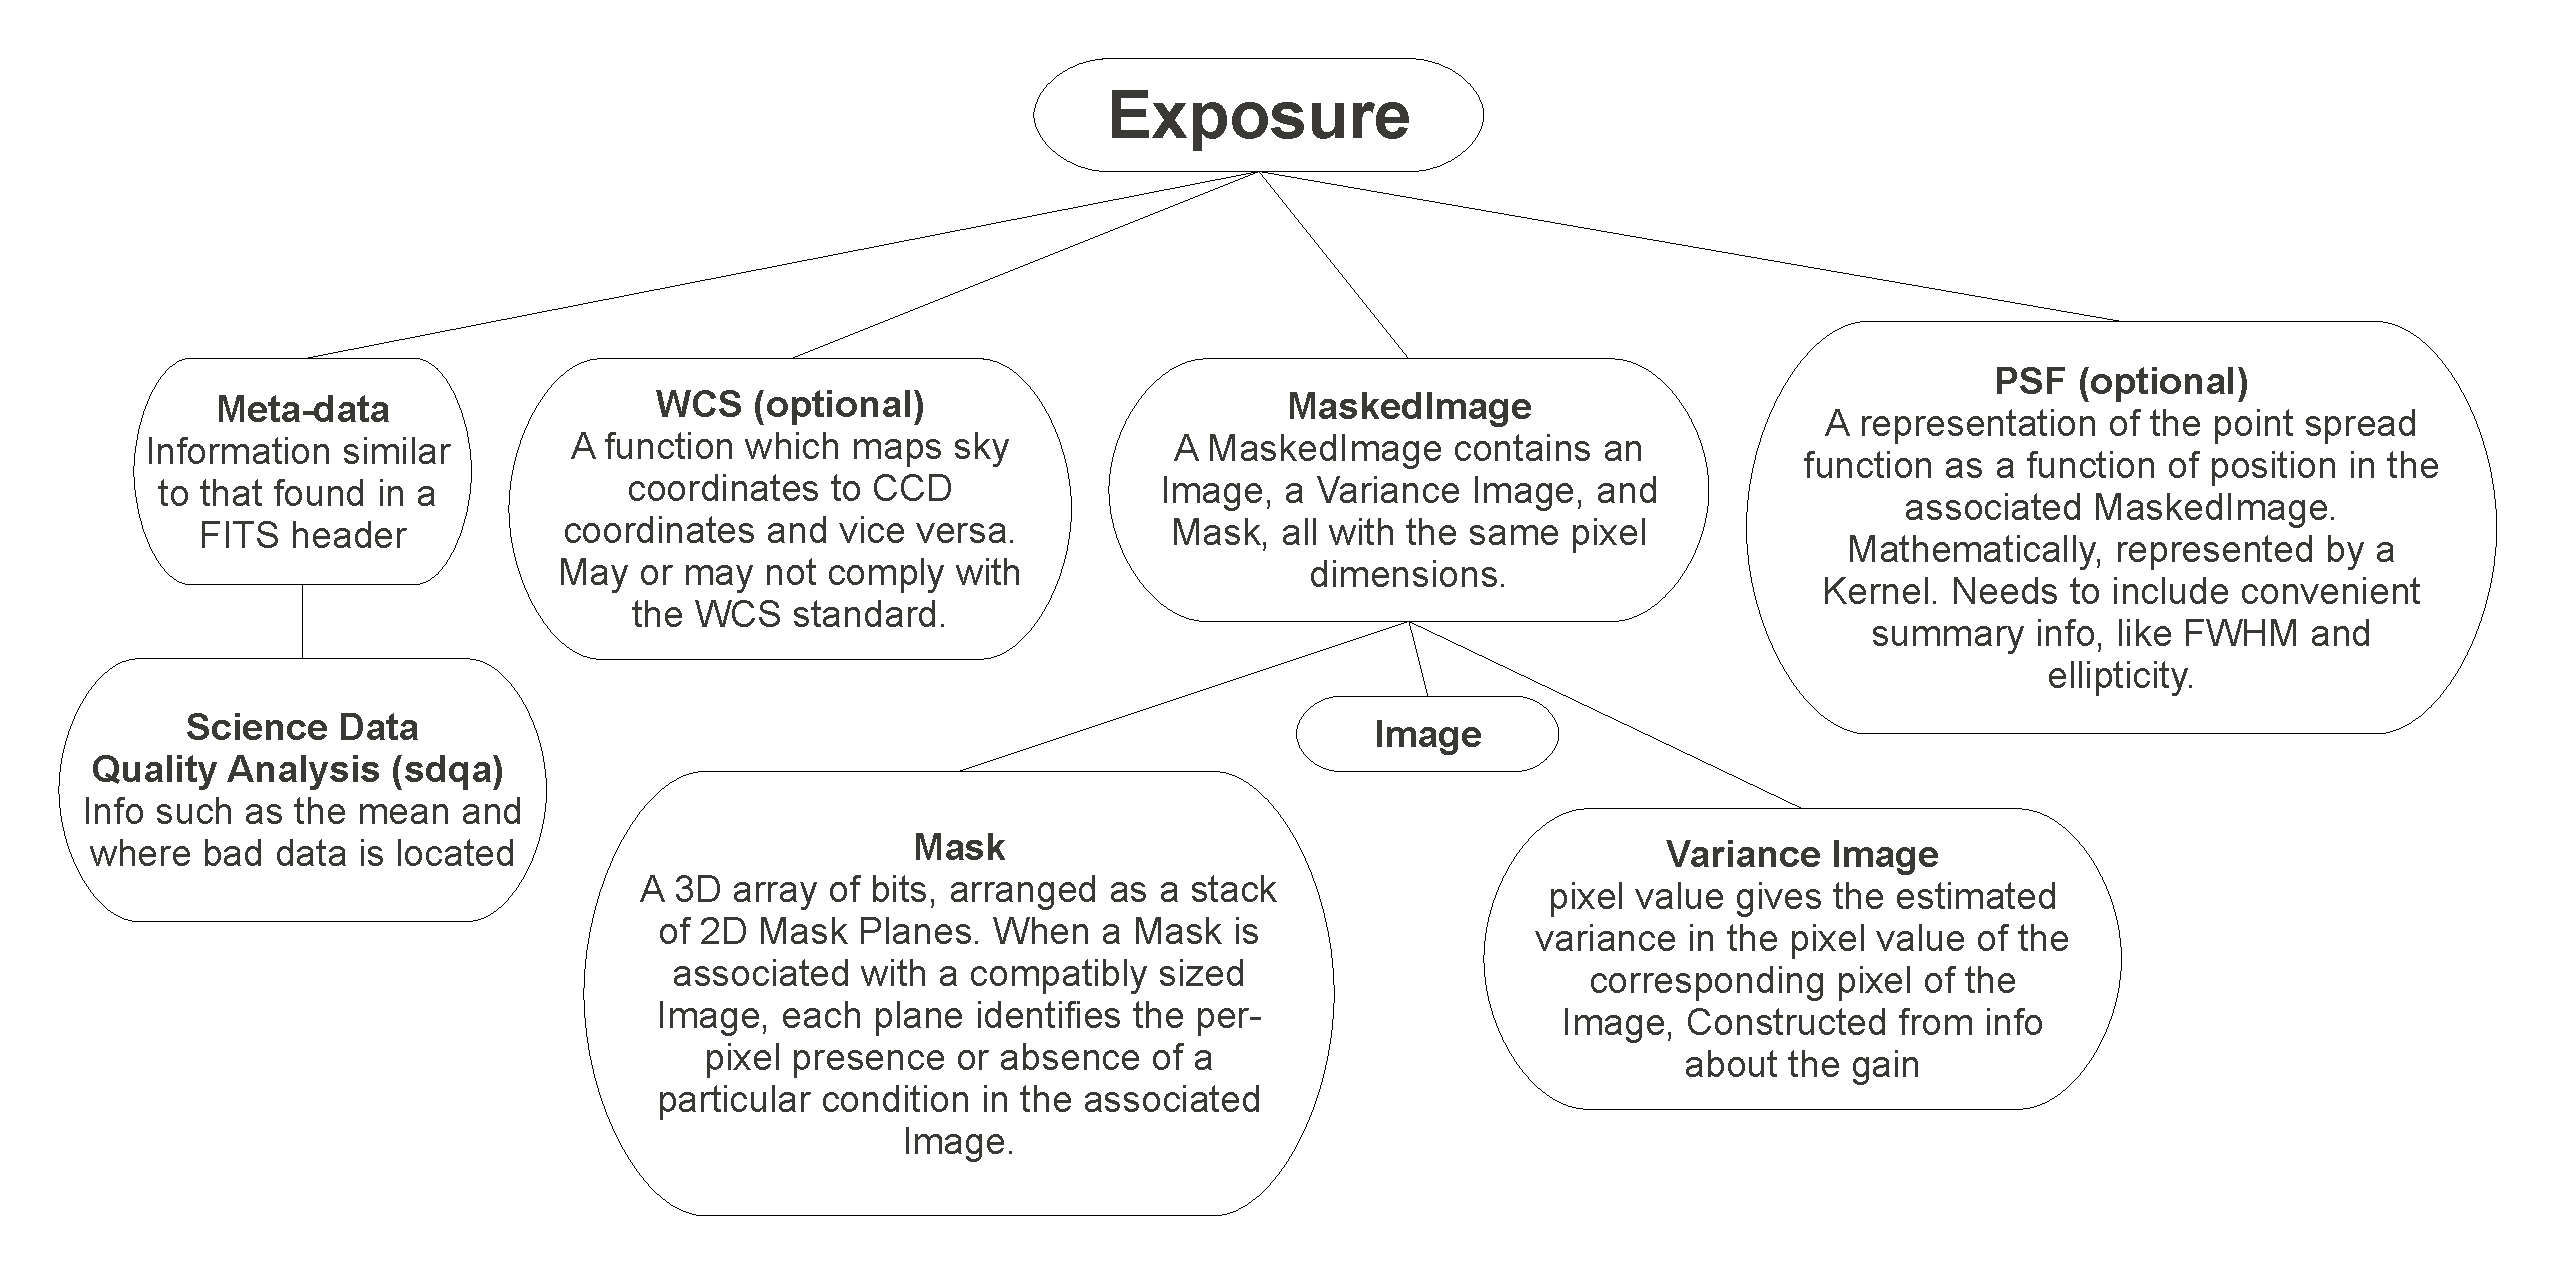
\includegraphics[angle=90,scale=0.5]{./figures/exposure.pdf}
%Not sure what to do with this, so it's on its side for now.



%See also the ``How to display an image'' link on the ``Related Pages''
%tab of the aforementioned documentation, for additional image
%commands.

